\section{Messungen}

Der erste Teil der Messungen untersucht stationäre Betriebsszustände, der zweite Teil untersucht das dynamische Verhalten der Strecke.

\subsection{Stationärer Zustand am Arbeitspunkt}
%Messen Sie mit einem elektronischen Temperaturfühler die Temperatur des Luftstroms am Arbeitspunkt in ◦C und notieren Sie die zugehörigen Werte der Messwertgeber (uyϑ0 , uyF0 ),nachdem sich der stationäare Zustand eingestellt hat.

%Wiederholen Sie die Messungen für 40%, 50% und 60% Heizleistung indem Sie für jede Heizleistung die LÜfterspannung auf 60%, 50% und 40% variieren.

Gemessen wurde die Ausgangsspannung des Temperatur- und des Luftstromsensors bei variierten Stellgraden für Heiz- und Lüfterleistung. Hierbei wurden die neun möglichen Kombination der Werte \(\SI{40}{\percent}\), \( \SI{50}{\percent}\) und \(\SI{60}{\percent}\) untersucht. Vor dem Ablesen der Werte wurde gewartet, bis diese sich stabilisieren. Die Messwerte sind in \autoref{tab:M1_12_werte} eingetragen.

\begin{table}[ht]
    \centering
    \begin{tabular}{|c|c|c|c|c|}\hline
    \tbf{Heizung}     & \tbf{Lüfter}  & \tbf{Temperatur}   & \tbf{Luftstrom}     & \tbf{Temperatur } \\ \hline
    \(u_{uP}\)                 & \(u_{uL}\)                & \(u_{y\vartheta}\)        & \(u_{yF}\)                & \(\vartheta\) \\ \hline
    \SI{4}{\volt}               & \SI{4}{\volt}             & \SI{3.7}{\volt}           & \SI{2.51}{\volt}          & \SI{41.3}{\celsius} \\ \hline
    \SI{5}{\volt}               & \SI{4}{\volt}             & \SI{4.37}{\volt}          & \SI{2.48}{\volt}          & \SI{44.4}{\celsius} \\ \hline
    \SI{6}{\volt}               & \SI{4}{\volt}             & \SI{4.97}{\volt}          & \SI{2.49}{\volt}          & \SI{47.2}{\celsius} \\ \hline
    \SI{4}{\volt}               & \SI{5}{\volt}             & \SI{3.23}{\volt}          & \SI{3.59}{\volt}          & \SI{39.1}{\celsius} \\ \hline
    \SI{5}{\volt}               & \SI{5}{\volt}             & \SI{3.76}{\volt}          & \SI{3.38}{\volt}          & \SI{41.7}{\celsius} \\ \hline
    \SI{6}{\volt}               & \SI{5}{\volt}             & \SI{4.34}{\volt}          & \SI{3.4}{\volt}           & \SI{44.3}{\celsius} \\ \hline
    \SI{4}{\volt}               & \SI{6}{\volt}             & \SI{3.06}{\volt}          & \SI{4.23}{\volt}          & \SI{38.4}{\celsius} \\ \hline
    \SI{5}{\volt}               & \SI{6}{\volt}             & \SI{3.48}{\volt}          & \SI{4.45}{\volt}          & \SI{40.3}{\celsius} \\ \hline
    \SI{6}{\volt}               & \SI{6}{\volt}             & \SI{3.96}{\volt}          & \SI{4.25}{\volt}          & \SI{42.6}{\celsius} \\ \hline
    \end{tabular}
    \caption{Sollwertkombinationen und resultierende Messwerte}
    \label{tab:M1_12_werte}
\end{table}


\subsection{Sprungantworten für Eingangssprünge der Heizleistung}

% Bei den nachfolgenden Oszillogrammen ist auf eine hohe Auflösung zu achten (größtmögliche Darstellung der Kurven). Um den kleinstmöglichen Messbereich am Oszilloskop wählen zu können, ist der Offset des aufzuzeichnenden Signales mit einer in Serie geschalteten externen Spannungsquelle zu kompensieren.

% Zeichnen Sie die Sprungantworten der Temperatur für Eingangssprünge der Heizleistung von 40% auf 60% und von 60% auf 40% auf.

% lüfter 5v
% auf 60 bzw 40 % einstellen
Für die Messung des dynamischen Verhaltens wird zunächst die Lüfterleistung auf \( \SI{50}{\percent} \) eingestellt. Anschließend wird die Heizleistung auf \( \SI{60}{\percent} \) eingestellt und gewartet, bis sich die Werte stabilisieren. Mithilfe eines externen Netzteil wird ein Offset auf die Ausgangsspannung des Temperatursensors gelegt, um die absolute Ausgangspannung zu reduzieren. Dadurch kann ein kleinerer Messbereich des Oszilloskops verwendet werden, was zu einer deutlichen Verbesserung der Auflösung führt.

In \autoref{fig:M1_3_a_step} und \autoref{fig:M1_3_a_step} sind die Sollwertsprünge und Sprungantworte der Regelstrecken abgebildet.

\newpage

\begin{figure}[H]
    \begin{center}
        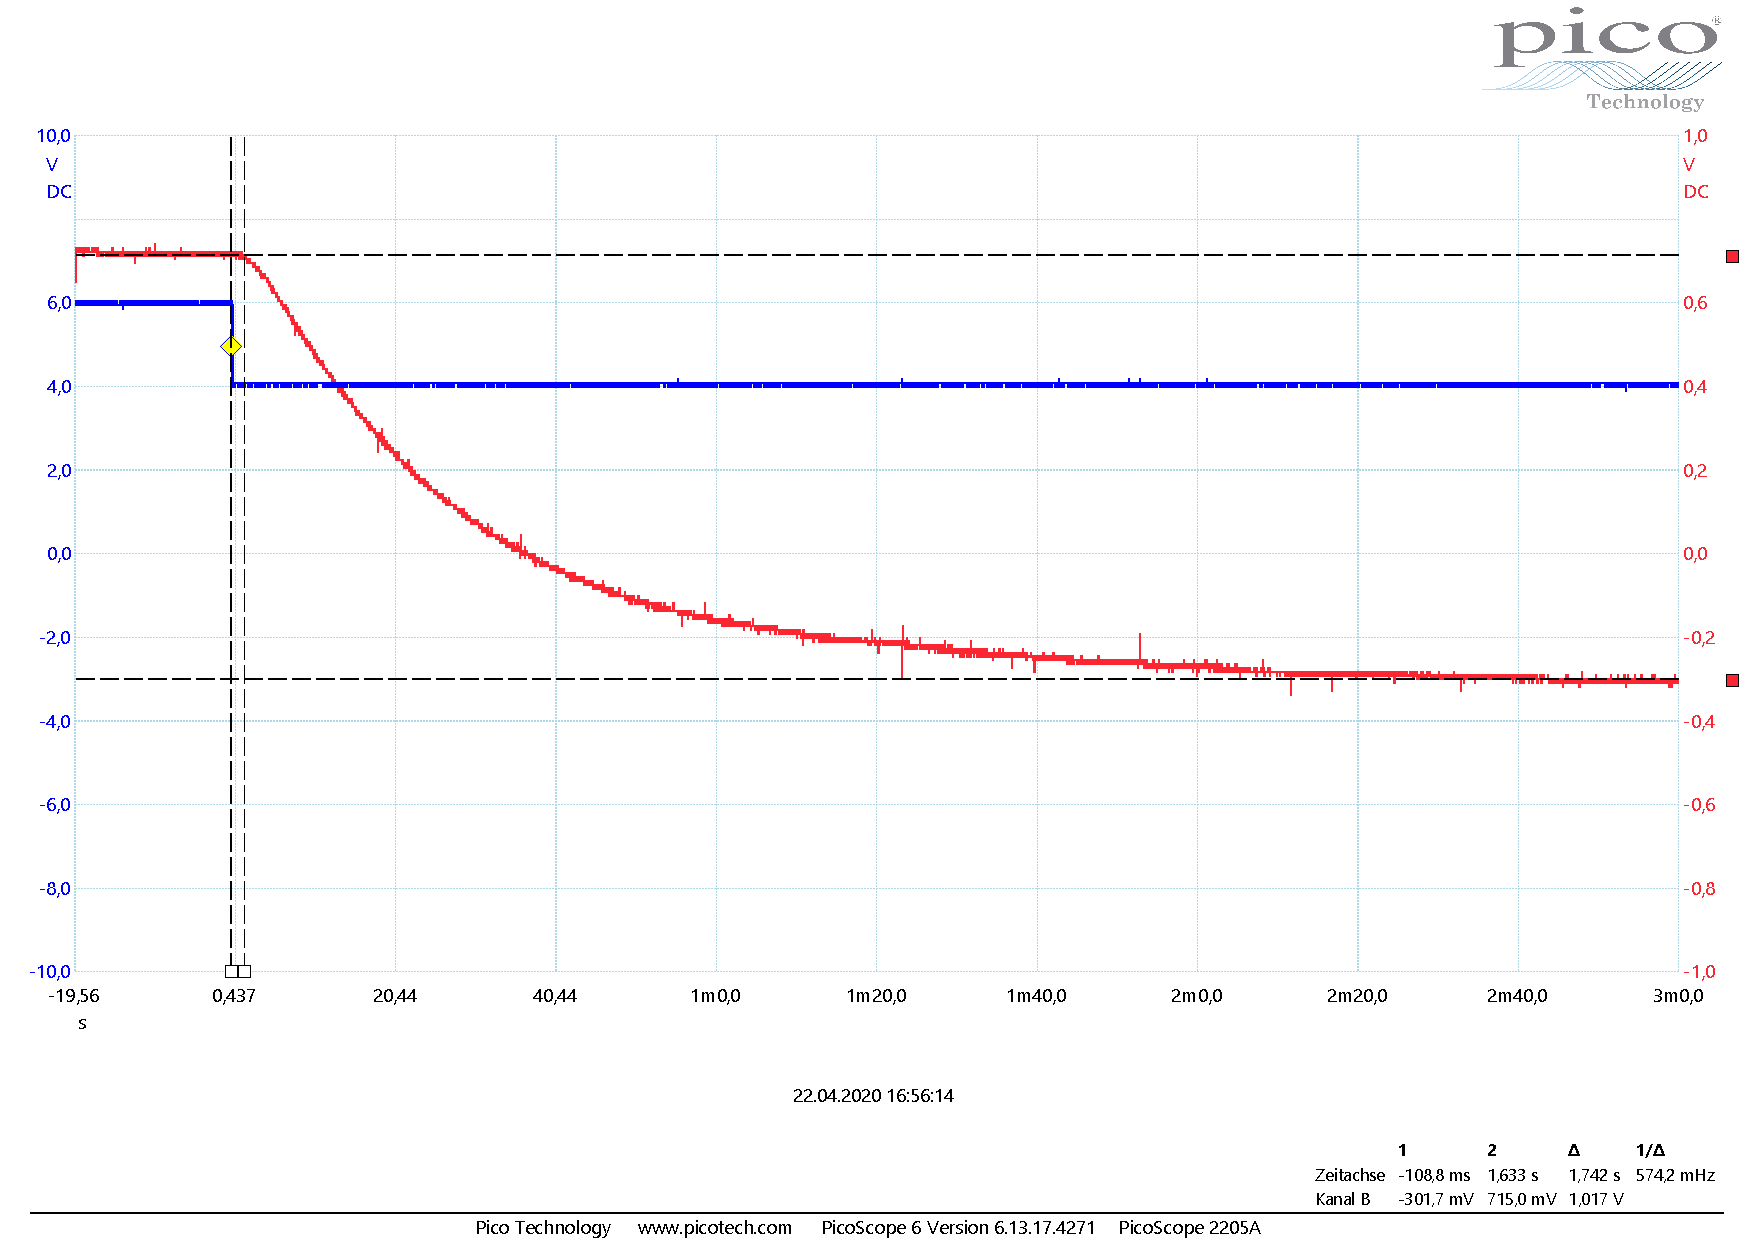
\includegraphics[width=0.85\textwidth]{pdf_ext/anlage5_messung1_u_uP_60_40.pdf}
        \caption{Sprungantwort bei Sollwertsprung von \( \SI{60}{\percent} \) auf \( \SI{40}{\percent} \)}
        \label{fig:M1_3_a_step}
    \end{center}
\end{figure}

\begin{figure}[H]
    \begin{center}
        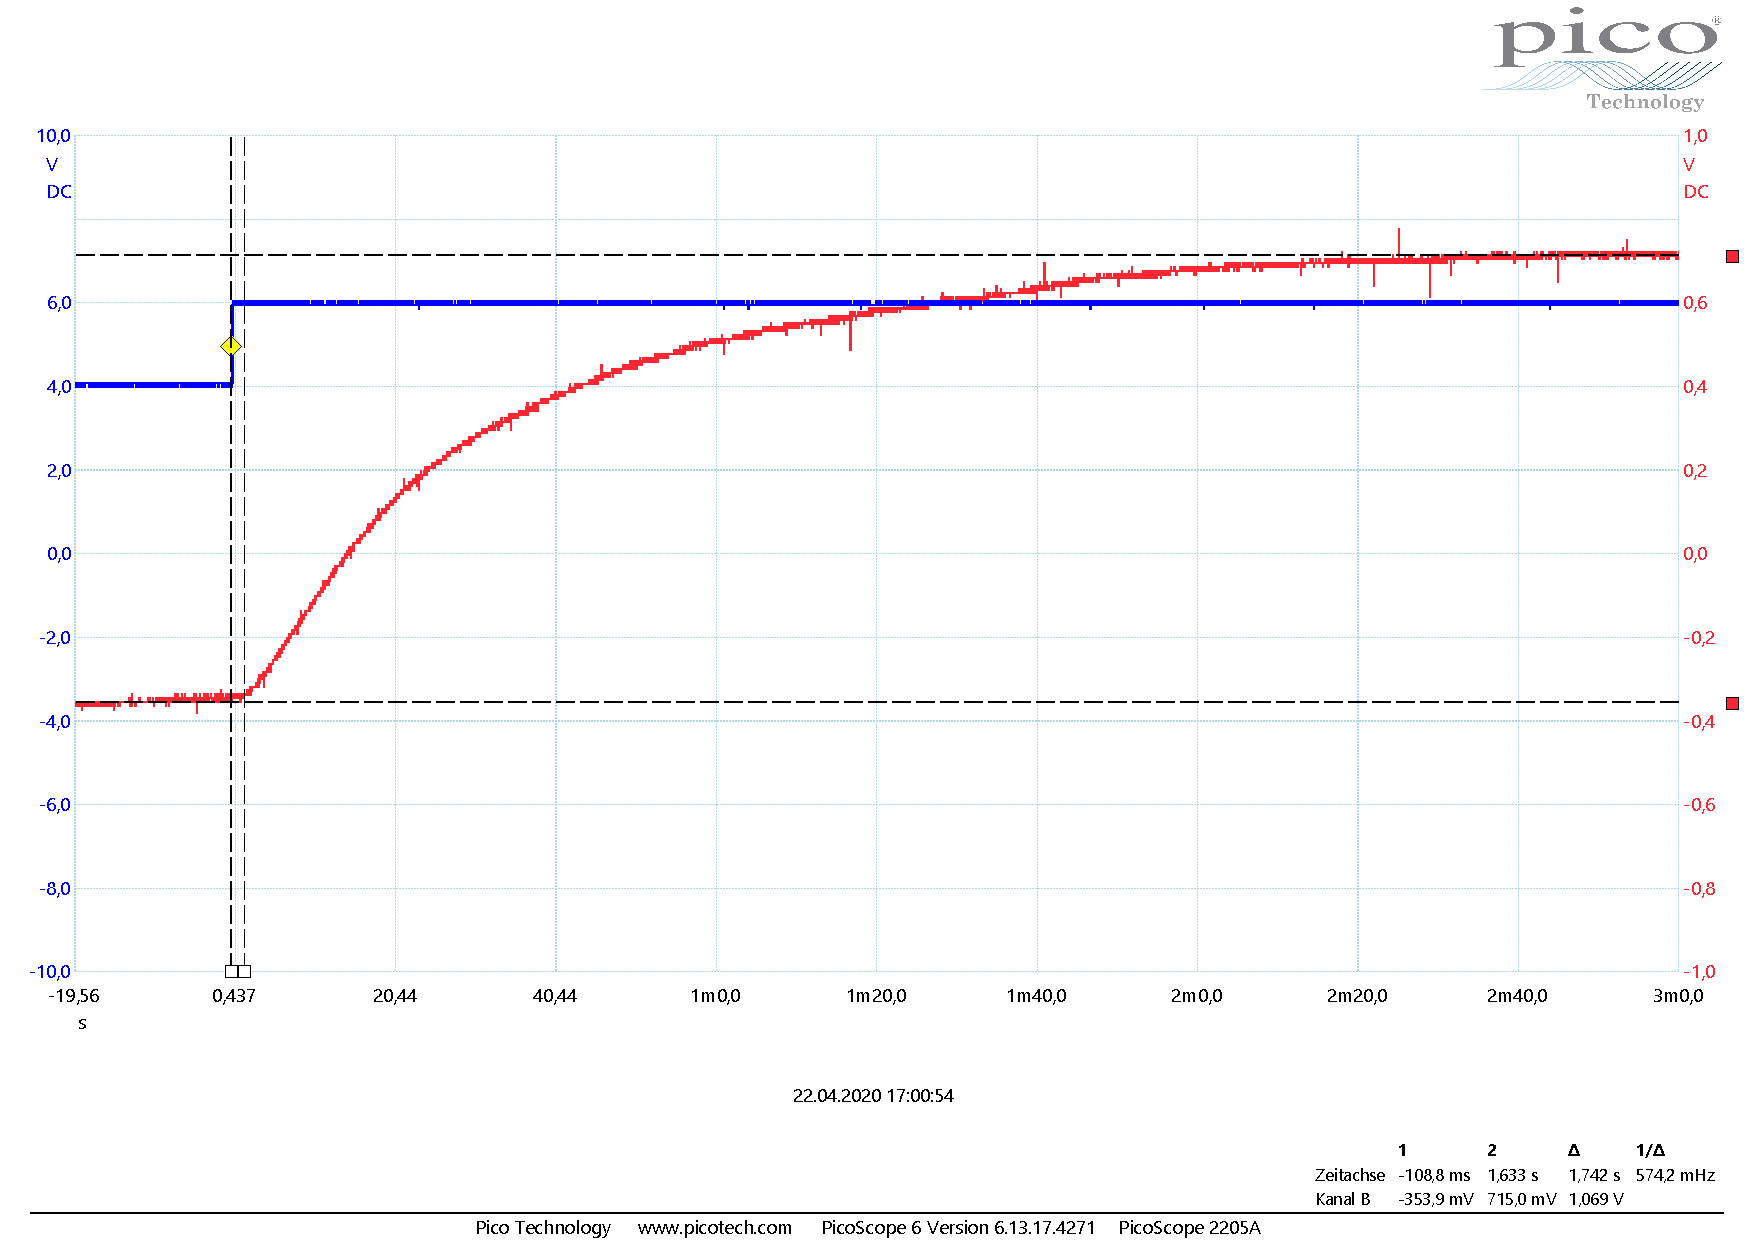
\includegraphics[width=0.85\textwidth]{pdf_ext/anlage5_messung2_u_uP_40_60.pdf}
        \caption{Sprungantwort bei Sollwertsprung von \( \SI{40}{\percent} \) auf \( \SI{60}{\percent} \)}
        \label{fig:M1_3_b_step}
    \end{center}
\end{figure}
 
 \newpage
 